\documentclass[border=10pt]{standalone}

\usepackage{tikz}
\usepackage{tikzsymbols}
\usetikzlibrary{calc,patterns,shapes.geometric}

\def\centerarc[#1](#2)(#3:#4:#5){\draw[#1] ($(#2)+({#5*cos(#3)},{#5*sin(#3)})$) arc (#3:#4:#5);}

\begin{document}
	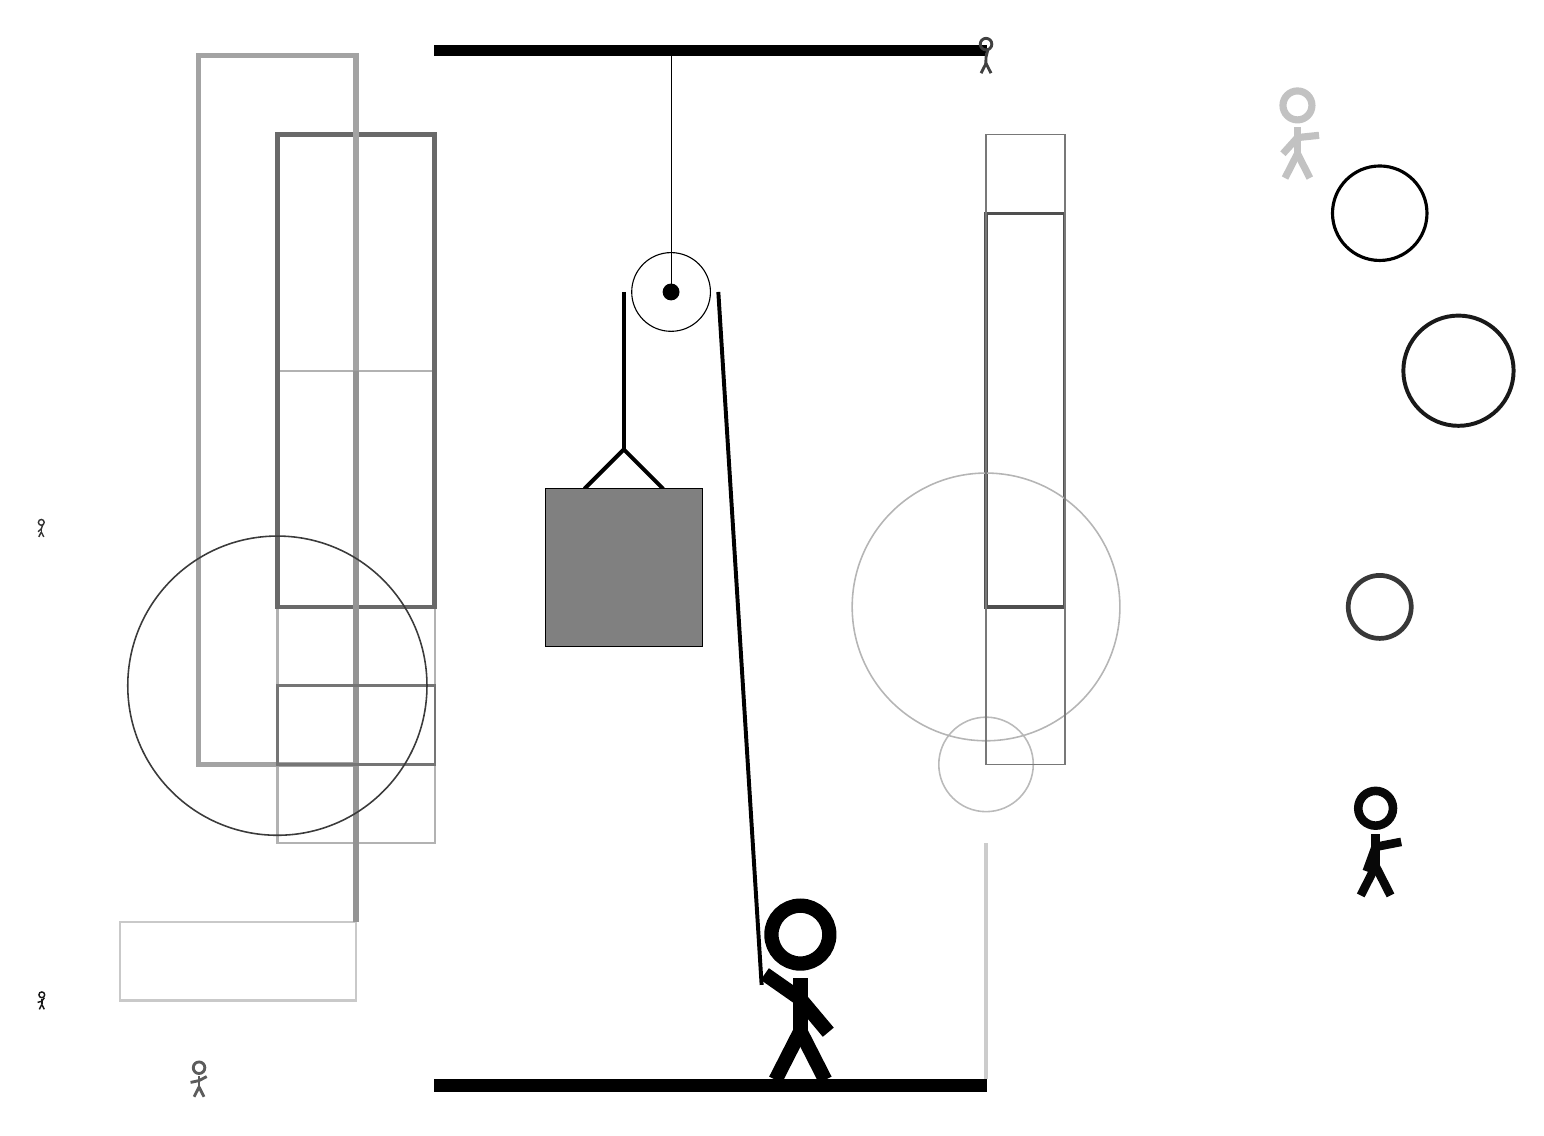
\begin{tikzpicture}
		%%%%% START %%%%%
		
		\draw[fill=black] (-2, 10) rectangle (5, 10.125);
		
		\draw (1, 7) circle (0.5);
		\draw[fill=black] (1, 7) circle (0.1);
		\draw (1, 10) -- (1, 7);
		
		\draw[line width=0.5mm] (-0.1, 4.5) -- (0.4, 5.0) -- (0.9, 4.5);
		\draw[fill=black!50] (-0.6, 4.5) rectangle (1.4, 2.5);
		
		\draw[line width=0.5mm] (0.4, 7) -- (0.4, 5.0);
		\centerarc[line width=0.5mm](1, 7)(0:180:0.6);
		\draw[line width=0.5mm](1.6, 7) -- (2.15, -1.8);
		
		\node at (2.6, -1.9) {\Strichmaxerl[10][-35][-50]};
		
		\draw[line width=0.4mm, color=black!69] (5, 3) rectangle (6, 8);
		
		\draw[line width=0.5mm, color=black!20](5, 0) -- (5, -3);
		\node[line width=0.4mm, color=black!80] at (-7, 4) {\Strichmaxerl[1][43][70]};
		\draw[line width=0.3mm, color=black!30] (-2, 0) rectangle (-4, 6);
		\draw [line width=0.2mm, color=black!27](5, 1) circle (0.6);
		\draw [line width=0.6mm, color=black!78](10, 3) circle (0.4);
		\draw [line width=0.2mm, color=black!29](5, 3) circle (1.7);
		
		\draw [line width=0.5mm, color=black!90](11, 6) circle (0.7);
		\draw[line width=0.6mm, color=black!59] (-4, 3) rectangle (-2, 9);
		
		\draw[line width=0.2mm, color=black!53] (5, 9) rectangle (6, 1);
		
		\node[line width=0.6mm, color=black!91] at (-7, -2) {\Strichmaxerl[1][15][54]};
		\draw[line width=0.3mm, color=black!21] (-3, -2) rectangle (-6, -1);
		\node[line width=0.2mm, color=black!97] at (10, 0) {\Strichmaxerl[6][70][11]};
		
		\draw[line width=0.7mm, color=black!36] (-3, 10) rectangle (-5, 1);
		\draw [line width=0.4mm, color=black!100](10, 8) circle (0.6);
		\draw[line width=0.7mm, color=black!42] (-3, 6) rectangle (-3, -1);
		
		\draw[line width=0.3mm, color=black!54] (-2, 1) rectangle (-4, 2);
		
		\node[line width=0.5mm, color=black!75] at (5, 10) {\Strichmaxerl[2][88][76]};
		\node[line width=0.7mm, color=black!64] at (-5, -3) {\Strichmaxerl[2][12][28]};
		\node[line width=0.5mm, color=black!24] at (9, 9) {\Strichmaxerl[5][48][6]};
		\draw [line width=0.2mm, color=black!77](-4, 2) circle (1.9);
		
		
		\draw[fill=black] (-2, -3) rectangle (5, -3.15);
		
		%%%%% END %%%%%
	\end{tikzpicture}
\end{document}